\documentclass[crop,tikz]{standalone}
\usetikzlibrary{calc}
\usepackage{graphicx}
\begin{document}
\begin{tikzpicture}
  \node[inner sep=0pt, anchor=north west] at (0,0)
    {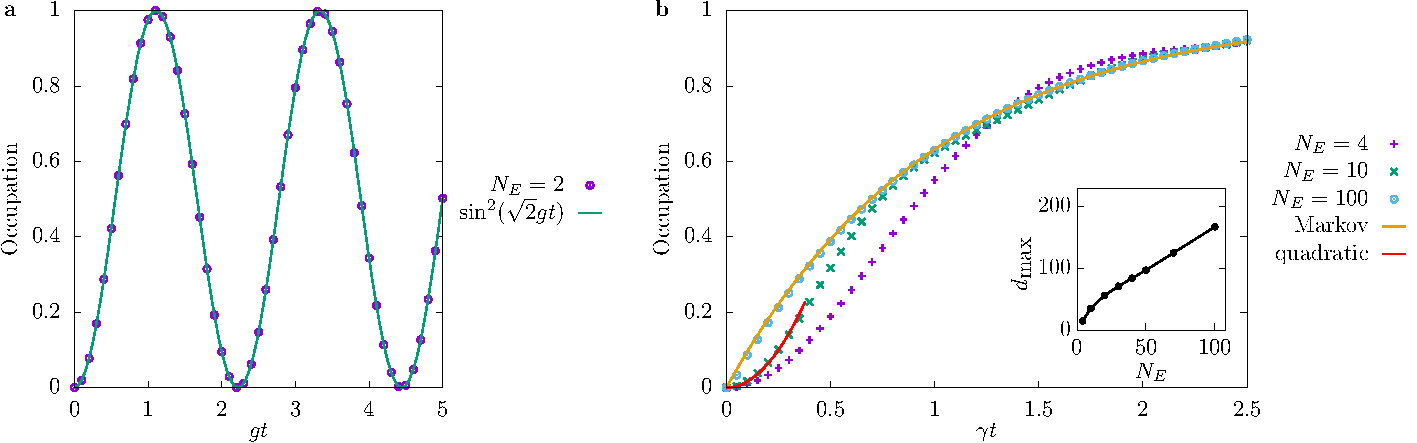
\includegraphics{fig2_data.pdf}};

  \node (inset) [inner sep=0pt, anchor=north west] at (1.4,-1.05) {};   %-0.96
  \fill [white, inner sep=0pt, anchor=north west, opacity=0.9] 
    ($(inset)+(0,0.15)$) rectangle ++ (4,-1.05);
%  \draw 
  \node[inner sep=0pt, anchor=north west] at (inset)
   {
\includegraphics[width=4cm]{chargetransfer_NE2.pdf}};

  \node[inner sep=0pt, anchor=north west] at (12.6,-0.4)       %-0.6 %-0.69
   {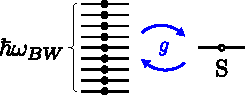
\includegraphics[width=4cm]{chargetransfer6.pdf}};

\end{tikzpicture}
\end{document}
